\section{Parallelism with Tasks}
To turn a Python function \verb|foo| into a “remote function” (a function that can be executed remotely and asynchronously), we declare the function with the \verb|@ray.remote| decorator. Then function invocations via \verb|f.remote()| will immediately return futures (a future is a reference to the eventual output), and the actual function execution will take place in the background (we refer to this execution as a task).

\inputminted{python}{../src/01.TaskParallelism.py}

Because the call to \verb|foo.remote(i)| returns immediately, four copies of \verb|foo| can be executed in parallel simply by running that line four times.

\subsection{Task Dependencies}
Tasks can also depend on other tasks. Below, the \verb|multiply_matrices| task uses the outputs of the two \verb|create_matrix| tasks, so it will not begin executing until after the first two tasks have executed. The outputs of the first two tasks will automatically be passed as arguments into the third task and the futures will be replaced with their corresponding values). In this manner, tasks can be composed together with arbitrary DAG dependencies.

\subsection{Aggregating Values Efficiently}
Task dependencies can be used in much more sophisticated ways. For example, suppose we wish to aggregate 8 values together. This example uses integer addition, but in many applications, aggregating large vectors across multiple machines can be a bottleneck. In this case, changing a single line of code can change the aggregation’s running time from linear to logarithmic in the number of values being aggregated.

\begin{figure}[!htbp]
    \centering
    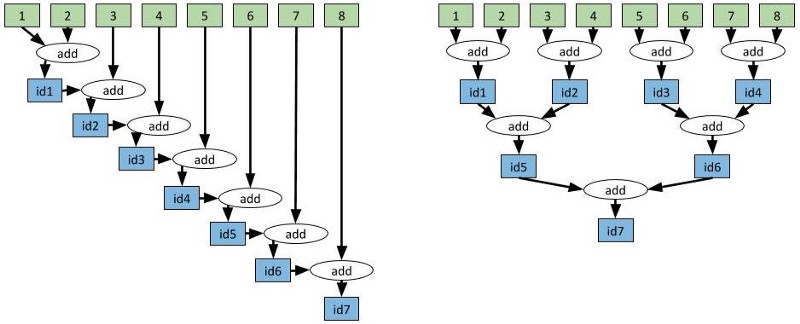
\includegraphics[width=\textwidth]{aggregating-values}
    \caption{The dependency graph on the left has depth 7. The dependency graph on the right has depth 3. The computations yield the same result, but the one on the right is much faster.}
\end{figure}

As described above, to feed the output of one task as an input into a subsequent task, simply pass the future returned by the first task as an argument into the second task. This task dependency will automatically be taken into account by Ray’s scheduler. The second task will not execute until the first task has finished, and the output of the first task will automatically be shipped to the machine on which the second task is executing.

\inputminted{python}{../src/03.ExplicitAggregation.py}

The above code is very explicit, but note that both approaches can be implemented in a more concise fashion using while loops.
